\documentclass{article}
\usepackage{fullpage,fourier,amsmath,amssymb}
\usepackage{wrapfig,listings,color,url}
\usepackage{xspace,epigraph, graphicx}
\usepackage{caption,subfig}
\usepackage[colorlinks=true,urlcolor=blue]{hyperref}

\title{Assignment 1 \\ Pass the Pigs}
\author{Prof. Darrell Long \\
CSE 13S -- Fall 2021}
\date{Due: October 3$^\text{rd}$ at 11:59\,pm}

\usepackage{fancyhdr}
\pagestyle{fancy}
\fancyhf{}

\fancypagestyle{plain}{%
  \fancyhf{}
  \renewcommand{\headrulewidth}{0pt}
  \renewcommand{\footrulewidth}{0pt}
  \lfoot{\textcopyright{} 2021 Darrell Long}
  \rfoot{\thepage}
}

\pagestyle{plain}

\definecolor{codegreen}{rgb}{0,0.5,0}
\definecolor{codegray}{rgb}{0.5,0.5,0.5}
\definecolor{codepurple}{rgb}{0.58,0,0.82}

\lstloadlanguages{C,make,python,fortran}

\lstdefinestyle{c99}{
    morekeywords={bool, uint8_t, uint16_t, uint32_t, uint64_t, int8_t, int16_t, int32_t, int64_t},
    commentstyle=\color{codegreen},
    keywordstyle=\color{magenta},
    numberstyle=\tiny\color{codegray},
    identifierstyle=\color{blue},
    stringstyle=\color{codepurple},
    basicstyle=\ttfamily,
    breakatwhitespace=false,
    breaklines=true,
    captionpos=b,
    keepspaces=true,
    numbers=left,
    numbersep=5pt,
    showspaces=false,
    showstringspaces=false,
    showtabs=false,
    tabsize=4
}

\newcommand{\monkey}[1]{
  \begin{center}
    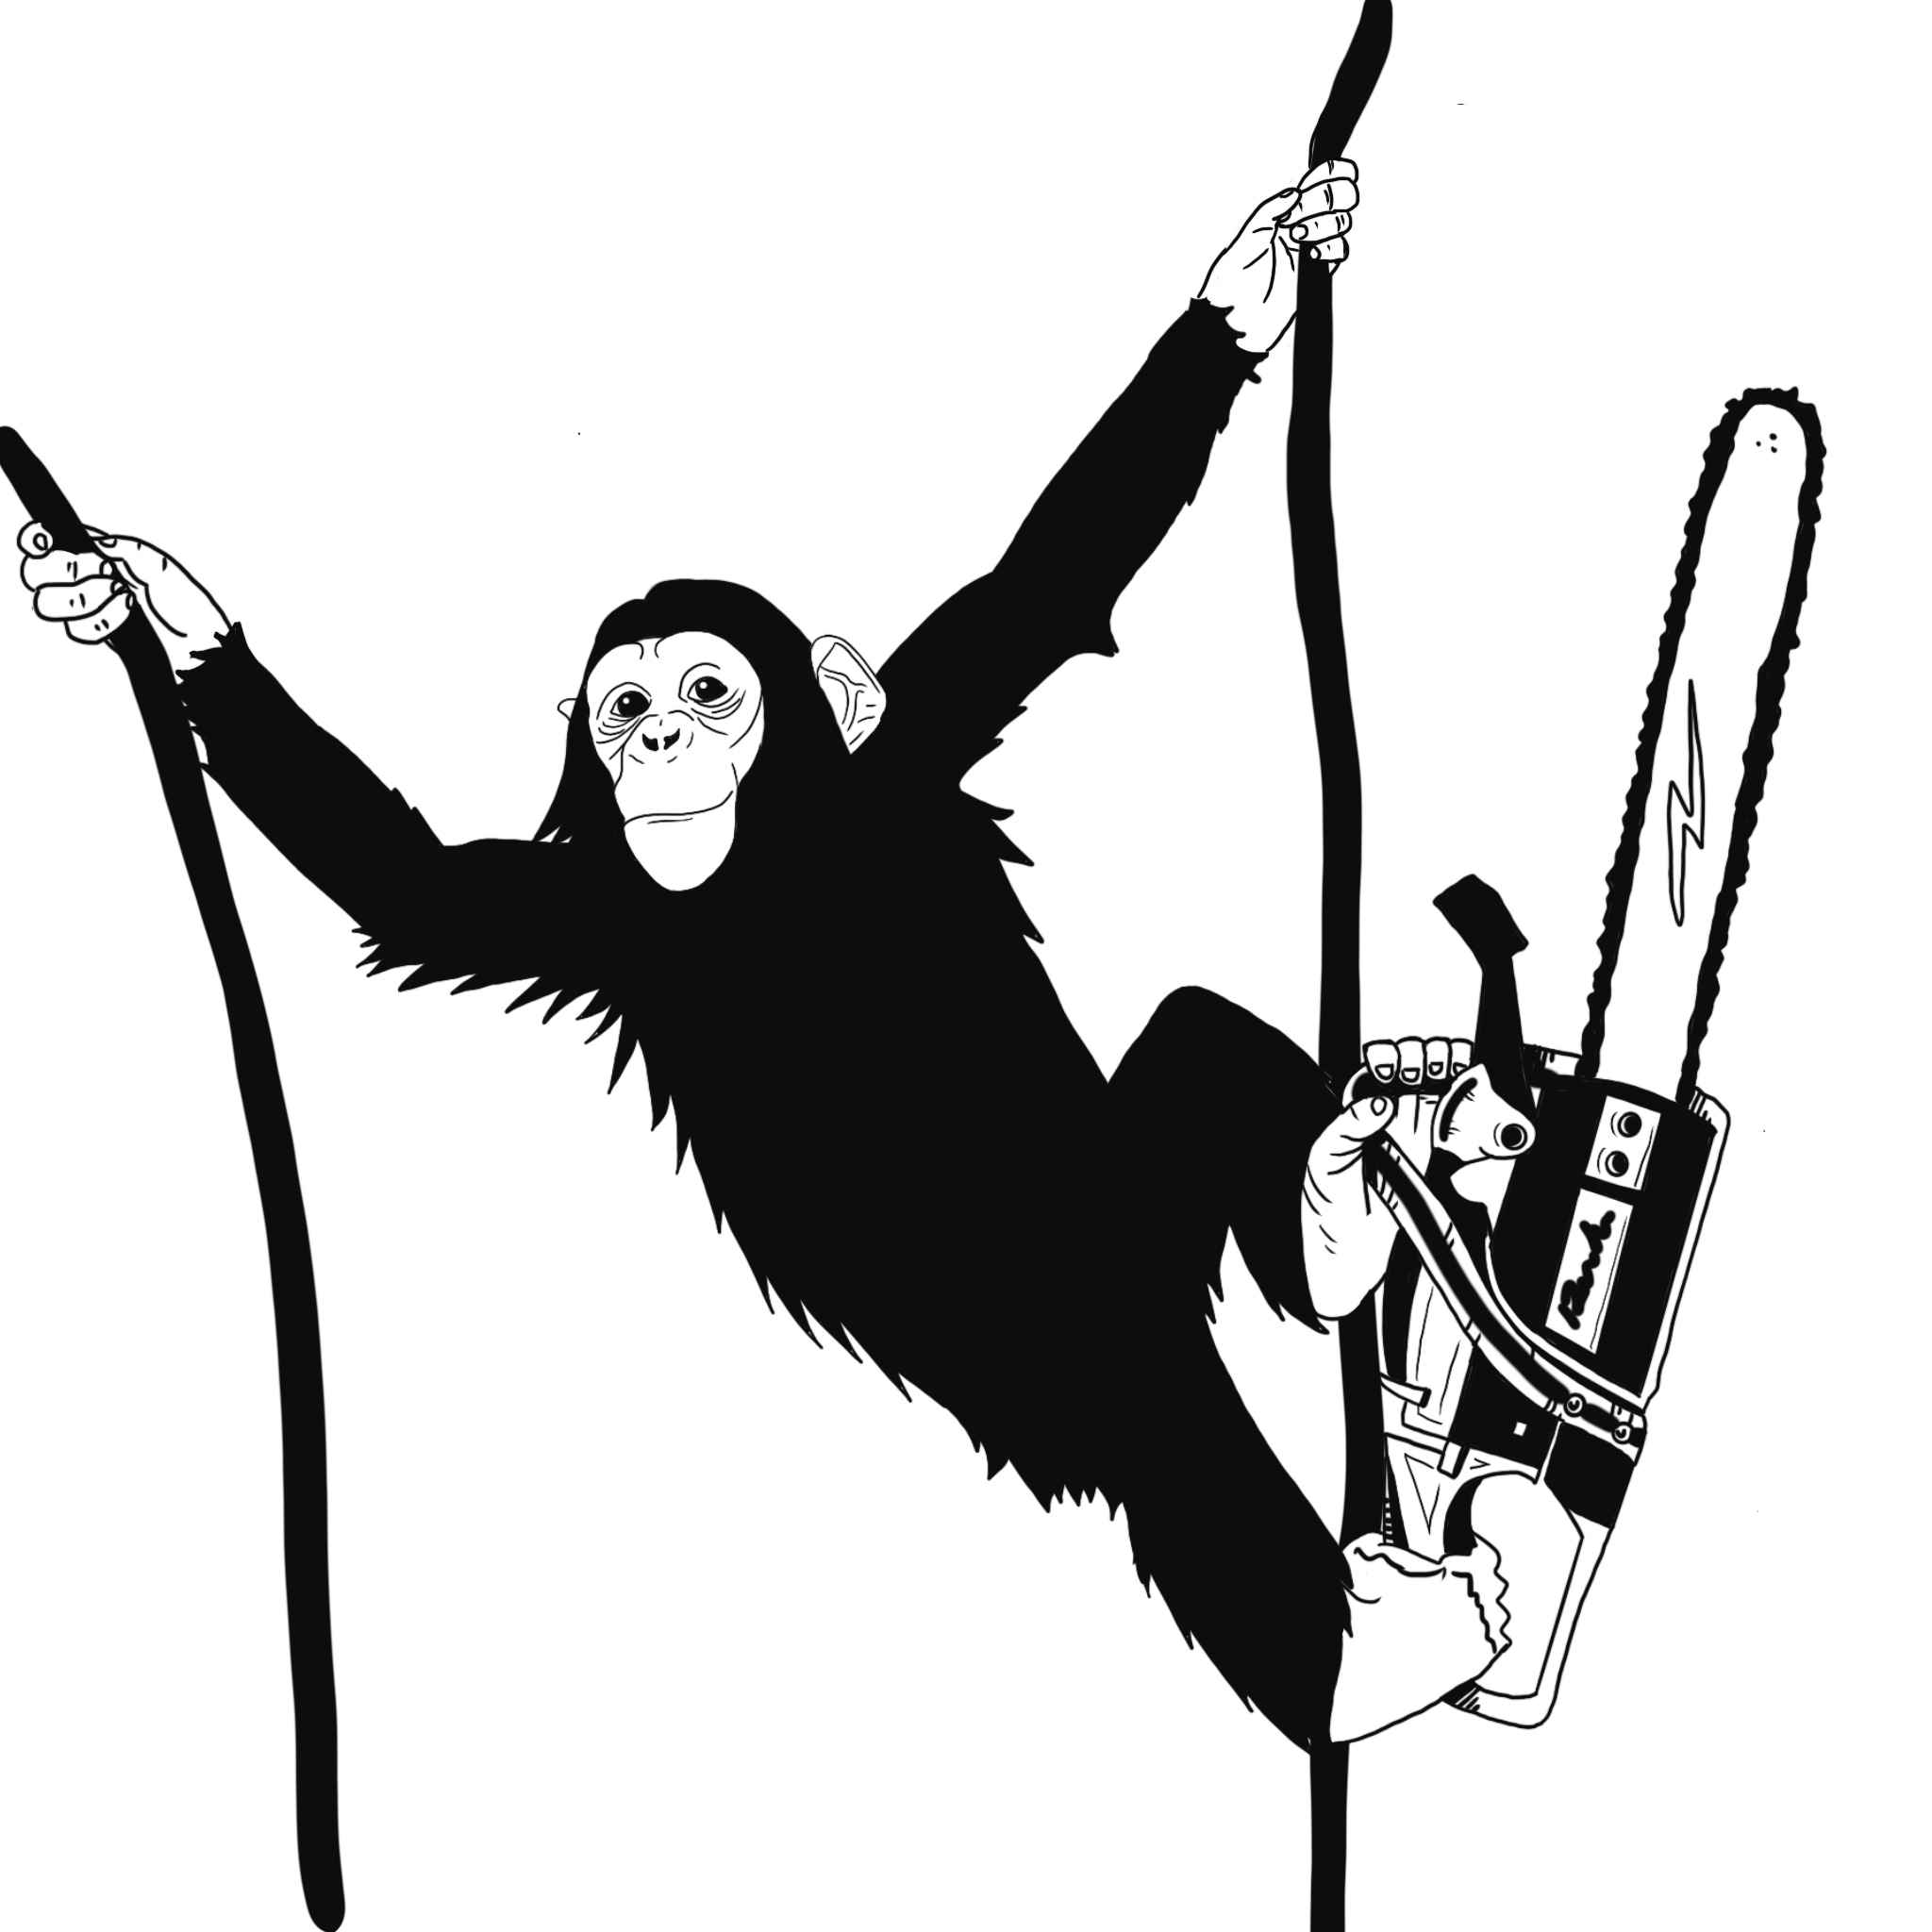
\includegraphics[width=0.35\textwidth]{../monkey.jpg} \\
    \emph{#1}
  \end{center}
}


\begin{document}

\maketitle

\begin{center}
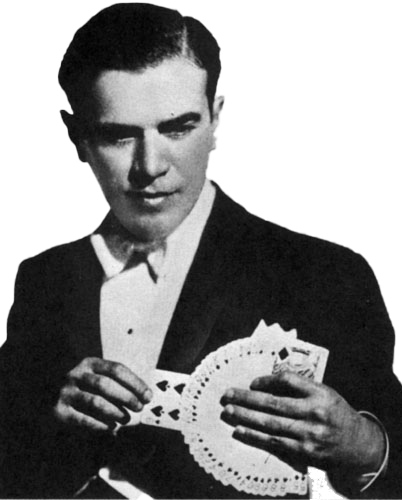
\includegraphics[width=0.2\textwidth]{./images/scarne.png} \\
John Scarne was an American magician who was adept at playing card manipulation.
\end{center}

\section{Introduction}

\epigraphwidth=0.67\textwidth \epigraph{\emph{The creatures outside
looked from pig to man, and from man to pig, and from pig to man again;
but already it was impossible to say which was which.}}{---George
Orwell, \emph{Animal Farm}}

\noindent We are going to implement a simplified version of David
Moffat's dice game\footnote{The traditional game\xspace
\emph{Pig} (\url{https://en.wikipedia.org/wiki/Pig_(dice_game)})
is played with a single six-sided die.
This simple dice game was first described in print by John Scarne in 1945.
Players take turns to roll a single die as many times as they wish,
adding all roll results to a running total, but losing their gained score for
the turn if they roll a $1$.
It has similarities with the traditional Mongolian game \emph{Shagai}\xspace
(\url{https://en.wikipedia.org/wiki/Shagai}).}
\emph{Pass the Pigs}. The game itself requires no
skill and no real decision-making, making it a great game for the
purpose of introductory programming in \textbf{C}. It will involve using
all the basic programming language facilities: primitive types, loops,
conditionals, arrays, and handling user input.

\section{The Rules of the Game}\label{rules}

\epigraphwidth=0.75\textwidth \epigraph{\emph{No one believes more
firmly than Comrade Napoleon that all animals are equal. He would be
only too happy to let you make your decisions for yourselves. But
sometimes you might make the wrong decisions, comrades, and then where
should we be?}}{---George Orwell, \emph{Animal Farm}}

\noindent The simplified version of \emph{Pass the Pigs} that we will
implement can be played with any $k$ players, such that $2 \le k \le
10$. The players are arranged in a cyclic fashion. The players will take
turns rolling an \emph{asymmetrical}\footnote{
        Shagai refers to the \emph{astragalus} of the ankle of a sheep or goat.
The bones are collected and used for traditional games and
fortune-telling throughout Central Asia, and games involving the
ankle bones may also be referred to by the name of the bones that are used.
Such bones have been used throughout
history, and are thought to be the first forms of dice.
}
die, affectionately named the \emph{pig},
to earn points. Rolling the pig can result in it landing in any of the
following positions:

\def\pigwidth{0.33\textwidth}
\begin{figure}
        \centering
        \subfloat[\textbf{Side}: Pig lands on one of its sides ($\frac{2}{7}$).]{%
                
\includegraphics[width=\pigwidth]{./images/side.jpg}}
                \hfill
        \subfloat[\textbf{Razorback}: Pig lands on its back ($\frac{1}{7}$).]{%
                
\includegraphics[width=\pigwidth]{./images/razorback.jpg}}
                \hfill
        \subfloat[\textbf{Trotter}: Pig lands upright ($\frac{1}{7}$).]{%
                
\includegraphics[width=\pigwidth]{./images/trotter.jpg}}
                \hfill
                \hbox{
        \subfloat[\textbf{Snouter}: Pig lands on its snout ($\frac{1}{7}$).]{%
                
\includegraphics[width=\pigwidth]{./images/snouter.jpg}}
                \quad
        \subfloat[\textbf{Jowler}: Pig lands on one of its ears ($\frac{2}{7}$).]{%
                
\includegraphics[width=\pigwidth]{./images/jowler.jpg}}
        }
        \caption{Scoring the pigs depends on how they land.}\label{fig:pigs}
\end{figure}

Rolling \textbf{Side} yields $0$ points and immediately ends the current
player's turn, resulting in the pig being passed to the next player in
the ring of players. Assuming $k$ players and $0$-based indexing, the next
player to go after player $0$ is player $1$. After player $1$ is player $2$.
Who is the
player after player $k - 1$? That would be player $0$.

Rolling either \textbf{Razorback} or \textbf{Trotter} earns $10$ points
for the player. Rolling \textbf{Snouter} earns $15$ points. Lastly,
rolling \textbf{Jowler} earns $5$ points. The game ends when any player
has earned $100$ or more points.

\section{Game Abstractions}

\epigraphwidth=0.33\textwidth \epigraph{\emph{All Animals Are Equal. But
Some Animals Are More Equal Than Others.}}{---George Orwell,
\emph{Animal Farm}}

\noindent
One of the most important skills to polish as Computer Scientists is
the ability to create abstractions for the problems that we need to
solve. In the case of ``Pass the Pigs,'' the most immediate problem is
to provide an abstraction for is the pig itself. Without some way of
representing the pig, and the rolling of the pig, we cannot even begin
to hope to implement the game in its entirety.

\subsection{Enumerating the Positions}\label{enum}

Your first thought might be to simply pseudorandomly generate a random
number $n$ such that $1 \le n \le 7$, then assign mappings from those
integers to each of the positions the pig can land in. Generating
pseudorandom numbers is required, but we will elect to use
\emph{enumerations} to represent each of the positions. Enumerations,
\texttt{enum} in \textbf{C}, are used to provide names for integer
constants. Using this, we can represent the positions and the pig in the
following manner:

\begin{clisting}{}
typedef enum { SIDE, RAZORBACK, TROTTER, SNOUTER, JOWLER } Position;
const Position pig[7] = {
  SIDE,
  SIDE,
  RAZORBACK,
  TROTTER,
  SNOUTER,
  JOWLER,
  JOWLER
};
\end{clisting}

The \texttt{typedef} is used to give a new name to a type. In this case,
we used \texttt{typedef} to name the enumeration of positions as
\texttt{Position}. The pig, then, can be represented as an \emph{array}
of positions. The act of ``rolling'' the pig can be achieved by randomly
selecting $1$ of the $7$ elements of the \texttt{pig} array.

\subsection{Generating Pseudorandom Numbers}
\epigraphwidth=0.45\textwidth
\epigraph{
\emph{Any one who considers arithmetical methods of producing random digits
is, of course, in a state of sin.}}{---John von Neumann, 1951}

\noindent
To generate pseudorandom numbers, the ones required to simulate the
rolling of the pig, you will need a \emph{pseudorandom number generator}
(PRNG). You will the utilize the one defined by the standard \textbf{C}
library (\texttt{libc}) which is interfaced with the two functions
\texttt{srandom()} and \texttt{random()}. You will need to include
\texttt{<stdlib.h>} in order to use these functions.

The \texttt{srandom()} function is essential in order to make your
program \emph{reproducible}. \texttt{srandom()} is used to \emph{set the
random seed}, which effectively establishes the start point of the
pseudorandom number sequence that is generated. This means, after
calling \texttt{srandom()} with a seed to set, that the pseudorandom
numbers that are generated with \texttt{random()} \emph{always} appear
in the same order. Try out the following snippet of code:

\begin{clisting}{}
#include <stdio.h>
#include <stdlib.h>

#define SEED 2021

int main(void) {
    for (int i = 0; i < 3; i += 1) {
        puts("Set the random seed.");
        srandom(SEED);
        for (int i = 0; i < 5; i += 1) {
            printf(" - generated %lu\n", random());
        }
    }
}
\end{clisting}

The output of running the pseudorandom number generation example is
given here so you can check if the numbers produced on your system
matches the ones produced by the system in which your program will be
graded on.

\begin{shlisting}{}
$ ./prng
Set the random seed.
 - generated 1644198542
 - generated 653251166
 - generated 273593510
 - generated 1964717451
 - generated 314322227
Set the random seed.
 - generated 1644198542
 - generated 653251166
 - generated 273593510
 - generated 1964717451
 - generated 314322227
Set the random seed.
 - generated 1644198542
 - generated 653251166
 - generated 273593510
 - generated 1964717451
 - generated 314322227
\end{shlisting}

\section{Your Task}

\epigraphwidth=0.4\textwidth \epigraph{\emph{``You have been my
friend,'' replied Charlotte, ``That in itself is a tremendous
thing.''}}{---E.B. White, \emph{Charlotte's Web}}

\noindent You will implement the version of \emph{Pass the Pigs} using
the rules presented in \S\ref{rules}, placing the implementation in the
source code file \texttt{pig.c}. The structure of your program should
follow these steps:

\begin{enumerate}
  \item Prompt the user to input the number of players, scanning in
    their input from \texttt{stdin}. You will want to use
    \texttt{scanf()} for this. To scan an \texttt{int} from
    \texttt{stdin}:

\begin{clisting}{}
int input = 0;
scanf("%d", &input);
\end{clisting}

    In the event that the user inputs anything other than a valid
    integer between $2$ and $10$ inclusive, print the following error to
    \texttt{stderr} informing them of improper program usage, then use
    the default value of $2$ as the number of players:

\begin{clisting}{}
fprintf(stderr, "Invalid number of players. Using 2 instead.\n");
\end{clisting}

    What are \texttt{stdin} and \texttt{stderr}? In \textsc{Unix}, every
    process on creation has access to the following input/output (I/O)
    streams: \texttt{stdin}, \texttt{stdout}, and \texttt{stderr}. A
    running program is a process. \texttt{stdin}, or \emph{standard
    input}, is the input stream in which data is sent to be read by a
    process. \texttt{stdout}, or \emph{standard output}, is the output
    stream where data written by a process is written to. The last
    stream, \texttt{stderr}, or \emph{standard error}, is an output
    stream like \texttt{stdout}, but is typically used for error
    messages.

  \item Prompt the user to input the random seed for this run of
    \emph{Pass the Pigs}. In the event that the user inputs anything
    other than a valid seed, print the following error to
    \texttt{stderr} informing them of improper program usage, the use
    the default value of 2021 as the random seed:

\begin{clisting}{}
fprintf(stderr, "Invalid random seed. Using 2021 instead.\n");
\end{clisting}

  \item Set the random seed and make sure that each
    player starts off with $0$ points. Note that it isn't made explicit
    how you keep track of each player's points. There are, of course,
    many ways to go about this. You are encouraged to keep things
    simple, however.

  \item Proceed around the circle starting from player $0$. For each
    player:
    \begin{enumerate}
      \item Print out the name of the player currently rolling the pig.
        An array of player names that you \emph{must use} will be
        provided in the header file \texttt{names.h}. Index $0$ of this
        names array is the name of the player $0$, index $1$ is the name of
        the player $1$, and so on and so forth.
      \item Roll the pig, increasing the player's point count until they
        either win the game or the pig lands on one of its two sides.
      \item If the player has greater or equal to $100$ points, then the
        win the game and a congratulatory message is printed to
        \texttt{stdout} celebrating their achievement.
      \item If the rolled pig lands on one of its two sides, then the
        player's turn ends and the next player in the circle gets to
        have their shot at rolling the pig.
    \end{enumerate}
\end{enumerate}

A working reference program, or \emph{binary}, can be found in the
course resources repository on \texttt{git.ucsc.edu}. It is also in this
repository that you will find the header file of player names,
\texttt{names.h}. \textcolor{red}{To receive full credit, the output of
your program \emph{must} match the output of the reference program.}

\section{Deliverables}
\epigraphwidth=0.25\textwidth
\epigraph{\emph{That'll do pig, that'll do.}}{---Farmer Hoggett, \emph{Babe}}

You will need to turn in the following source code and header files:

\begin{enumerate}
  \item \texttt{names.h}: This contains the array of player names to be
    used in your implementation of the game. This file will be provided
    in the course resource repository and \emph{may not} be modified.
  \item \texttt{pig.c}: This contains the implementation of the game.
\end{enumerate}

You will also need to turn in the following:

\begin{enumerate}
  \item \texttt{Makefile}:
    This file will be provided in the course resource repository. It is
    a file that directs program compilation, building the program
    \texttt{pig} from \texttt{pig.c}. Make sure to attend section to
    learn about using a \texttt{Makefile} and how to write your own.
  \item \texttt{README.md}: This must use proper Markdown syntax. It
    must describe how to use your program. Note down any known bugs or
    errors in this file as well for the graders.
  \item \texttt{DESIGN.pdf}: This document \emph{must} be a proper
    PDF\@. This design document must describe your design and design
    process for your program with enough detail such that a sufficiently
    knowledgeable programmer would be able to replicate your
    implementation. \textcolor{red}{This does not mean copying your
    entire program in verbatim}. You should instead describe how your
    program works with supporting pseudocode.
\end{enumerate}

\section{Submission}

\epigraphwidth=0.67\textwidth \epigraph{\emph{This work was strictly
voluntary, but any animal who absented himself from it would have his
rations reduced by half.}}{---George Orwell, \emph{Animal Farm}}

\noindent
Refer back assignment 0 for the instructions on how to properly submit
your assignment through \texttt{git}. Remember: \emph{add},
\emph{commit}, and \emph{push}!.

\textcolor{red}{Your assignment is turned in \emph{only} after you have
pushed and submitted the commit ID you want graded on Canvas. ``I
forgot to push'' and ``I forgot to submit my commit ID'' are not valid
excuses. It is \emph{highly} recommended to commit and push your changes
\emph{often}.}

\section{Supplemental Readings}

\begin{itemize}
  \item \textit{The C Programming Language} by Kernighan \& Ritchie
  \begin{itemize}
    \item Chapters 2 -- 4
    \item Chapter 7 \S 7.2, \S 7.4, \S 7.6
    \item \texttt{man 3 random}
    \item \texttt{man 3 printf}
  \end{itemize}
\end{itemize}

\monkey{I learned long ago, never to wrestle with a pig. You get dirty,
and besides, the pig likes it. \emph{---George Bernard Shaw}}

\end{document}
